\section{Technical Solution}
\subsection{Set-up}
The web-cam we have used to gather our data with is a Genius iSlim 321R that can take both regular and infra-red images.
Mounted to the web-cam is a plastic frame with 4 LED lights and 4 infra-red lights that are placed just besides the LED lights.
The LED and infra-red lights are controlled by a Phidget single board computer. %reference?
The LED lights have colours and are placed in the following pattern: Yellow-Red-Camera-Green-Yellow.
The web-cam set up can be seen on figure \ref{fig:webcam}.
\begin{figure}
\centering
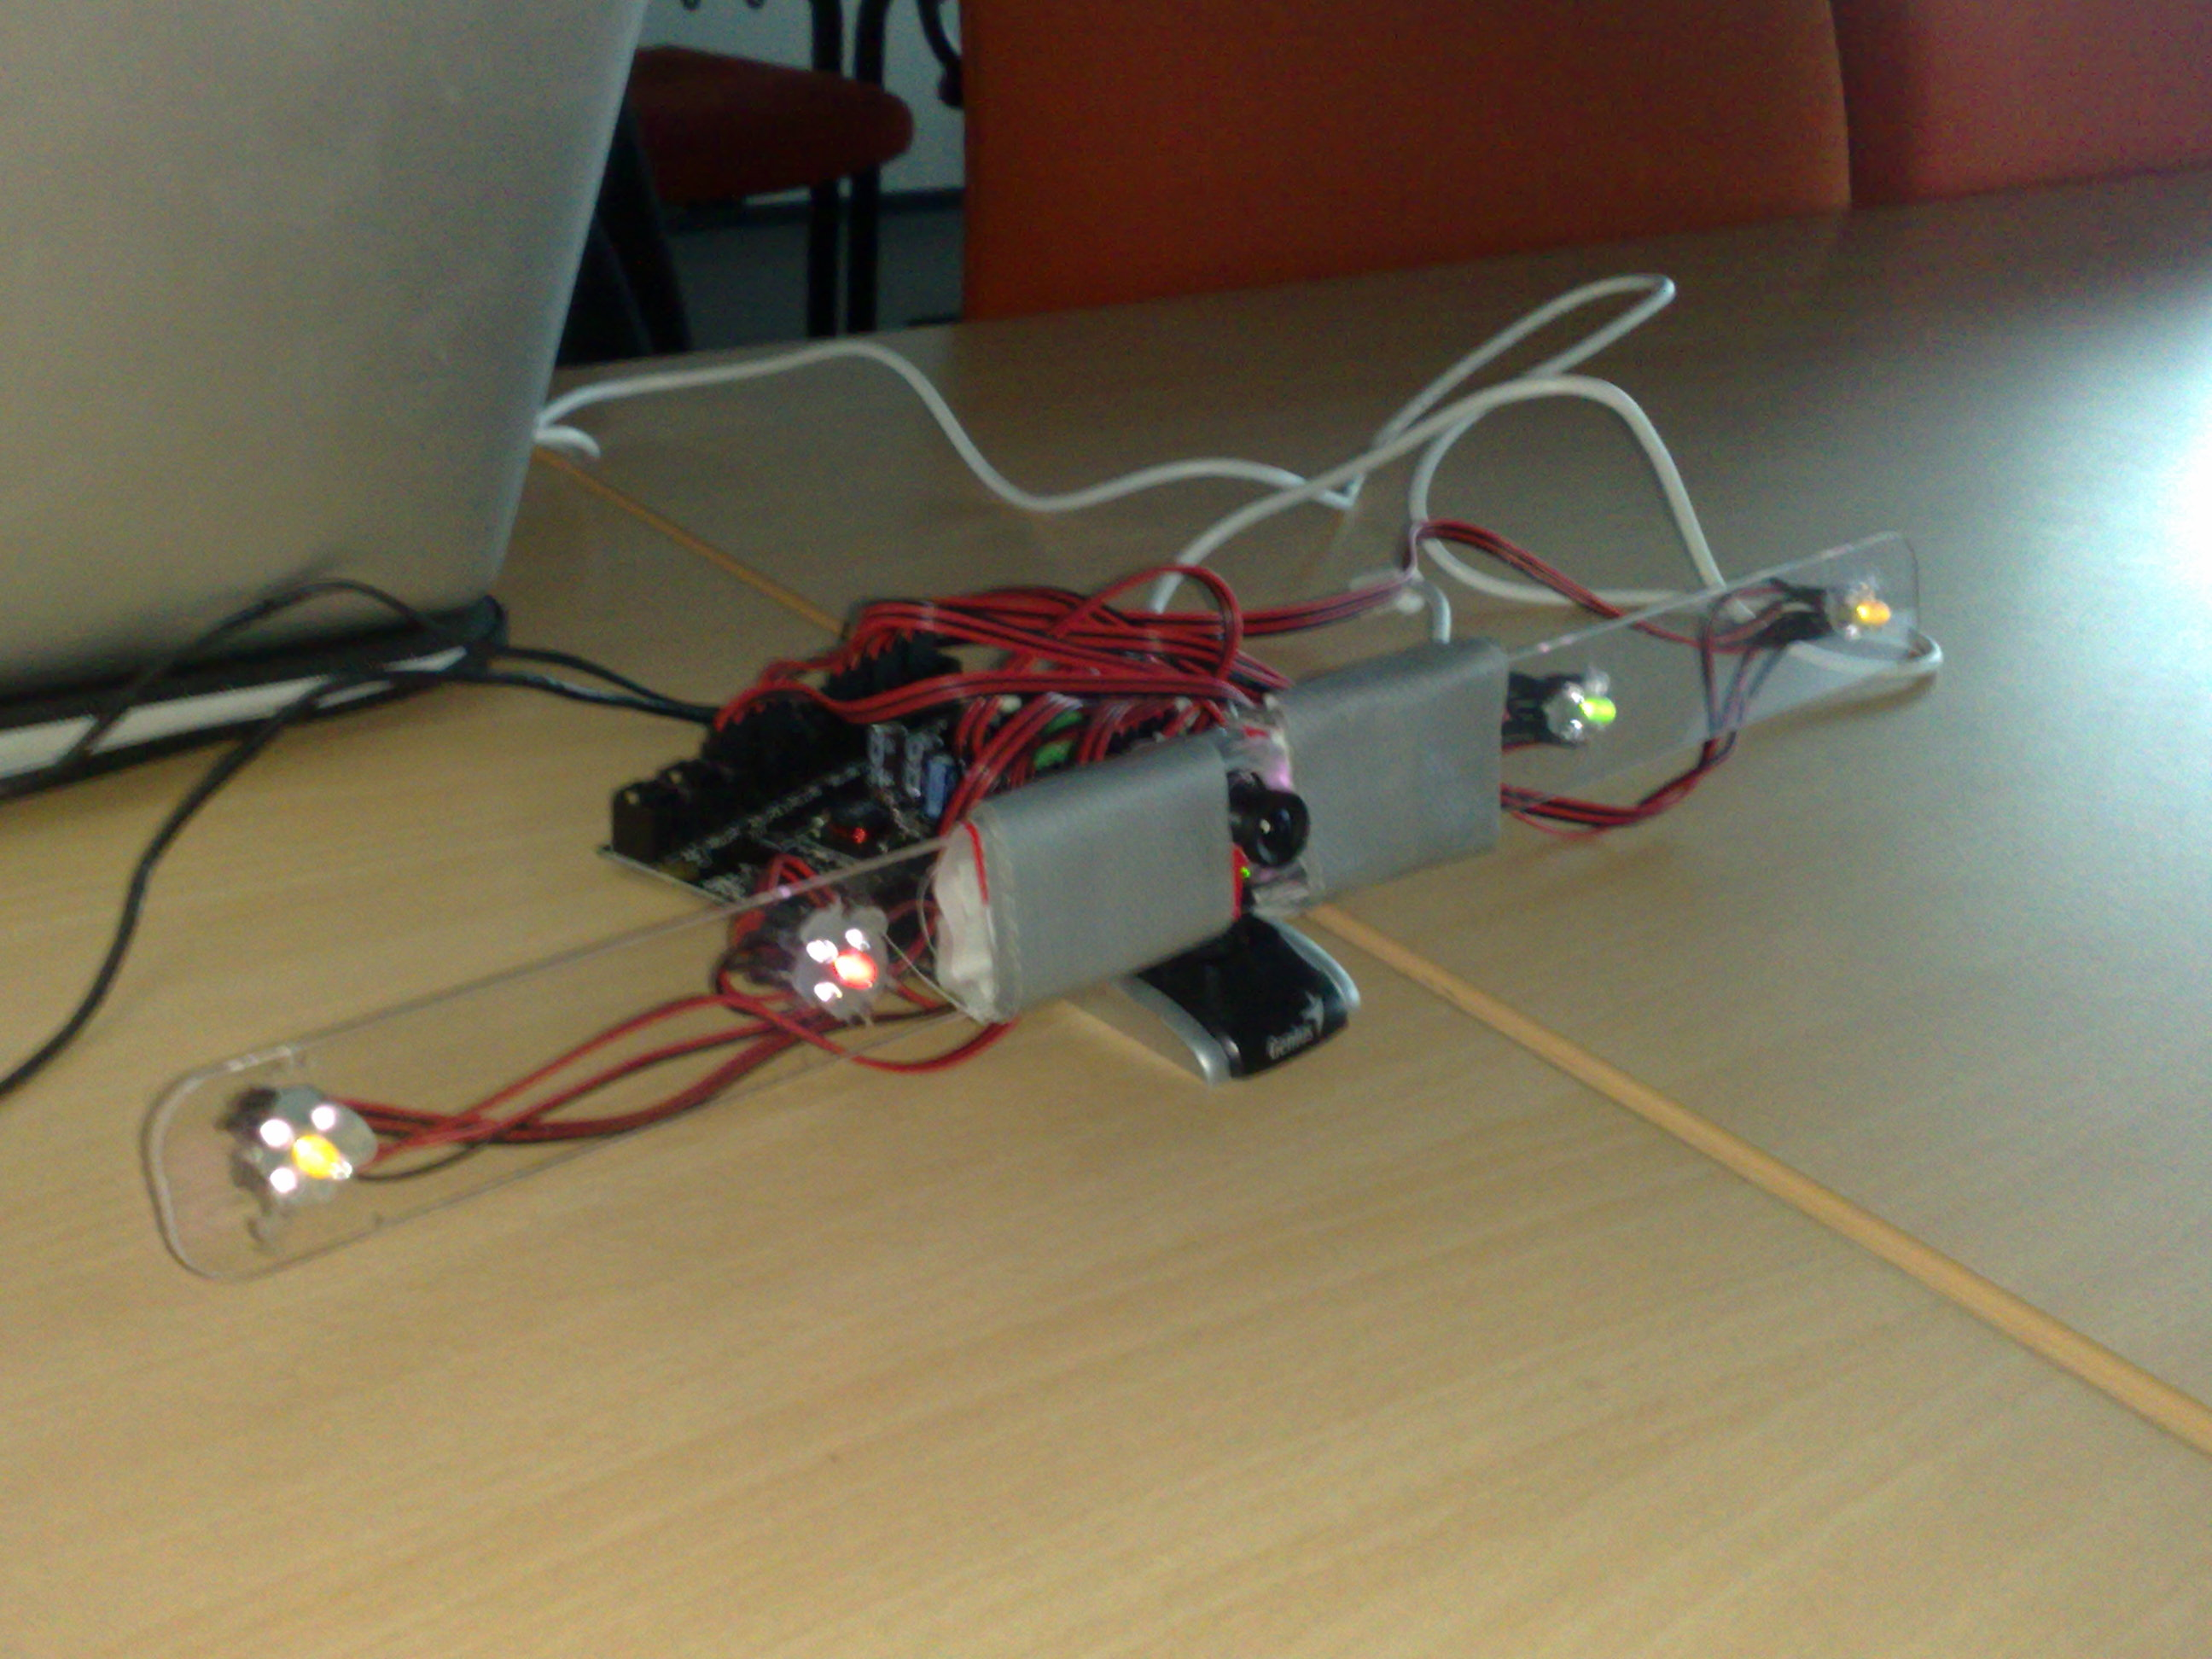
\includegraphics[width=0.8\textwidth]{cameratest}
\caption{Web-cam with mounted LED and infra-red lights.}
\label{fig:webcam}
\end{figure}

Our project is written in python 2.7 using the following libraries: 
\begin{itemize} %references?
\item{Scitkit-learn for machine learning algorithms.}
\item{OpenCV for image analysis and manipulation.}
\item{Numpy for matrix manipulation, also required by some of the other libraries.}
\item{Matplotlib for plotting results.}
\item{Phidgets python API to control the LED- and infra-red lights.}
\end{itemize}

To control the mounted lights, we modified a phidgets script by Adam Stelmack. See LED-simple.py for details. %proper reference?

\subsection{Experiment}
To perform the actual experiment, first of all data must be gathered.
The initial scenarios we wanted to test were combinations of the head being fixated and looking at a point, the head moving while looking at a point, and the infra-red lights being turned on or off.
This leaves us with the 4 scenarios with-light-head-move (WLHM), no-lights-head-move (NLHM), with-lights-head-still (WLHS) and no-lights-head-still (NLHS).
Test-subjects were then asked to place their head at a set point and look at the different points. For images of our test-subjects, see figures \ref{fig:mikkertest}, \ref{fig:mikkertest2}, \ref{fig:spencertest}, \ref{fig:petertest} and \ref{fig:nielstest}.
We then recorded video sequences of about 5 seconds in length at 30 frames per second of the various scenarios and saved the videos with appropriate names according to the scenarios.

\begin{figure}
\centering
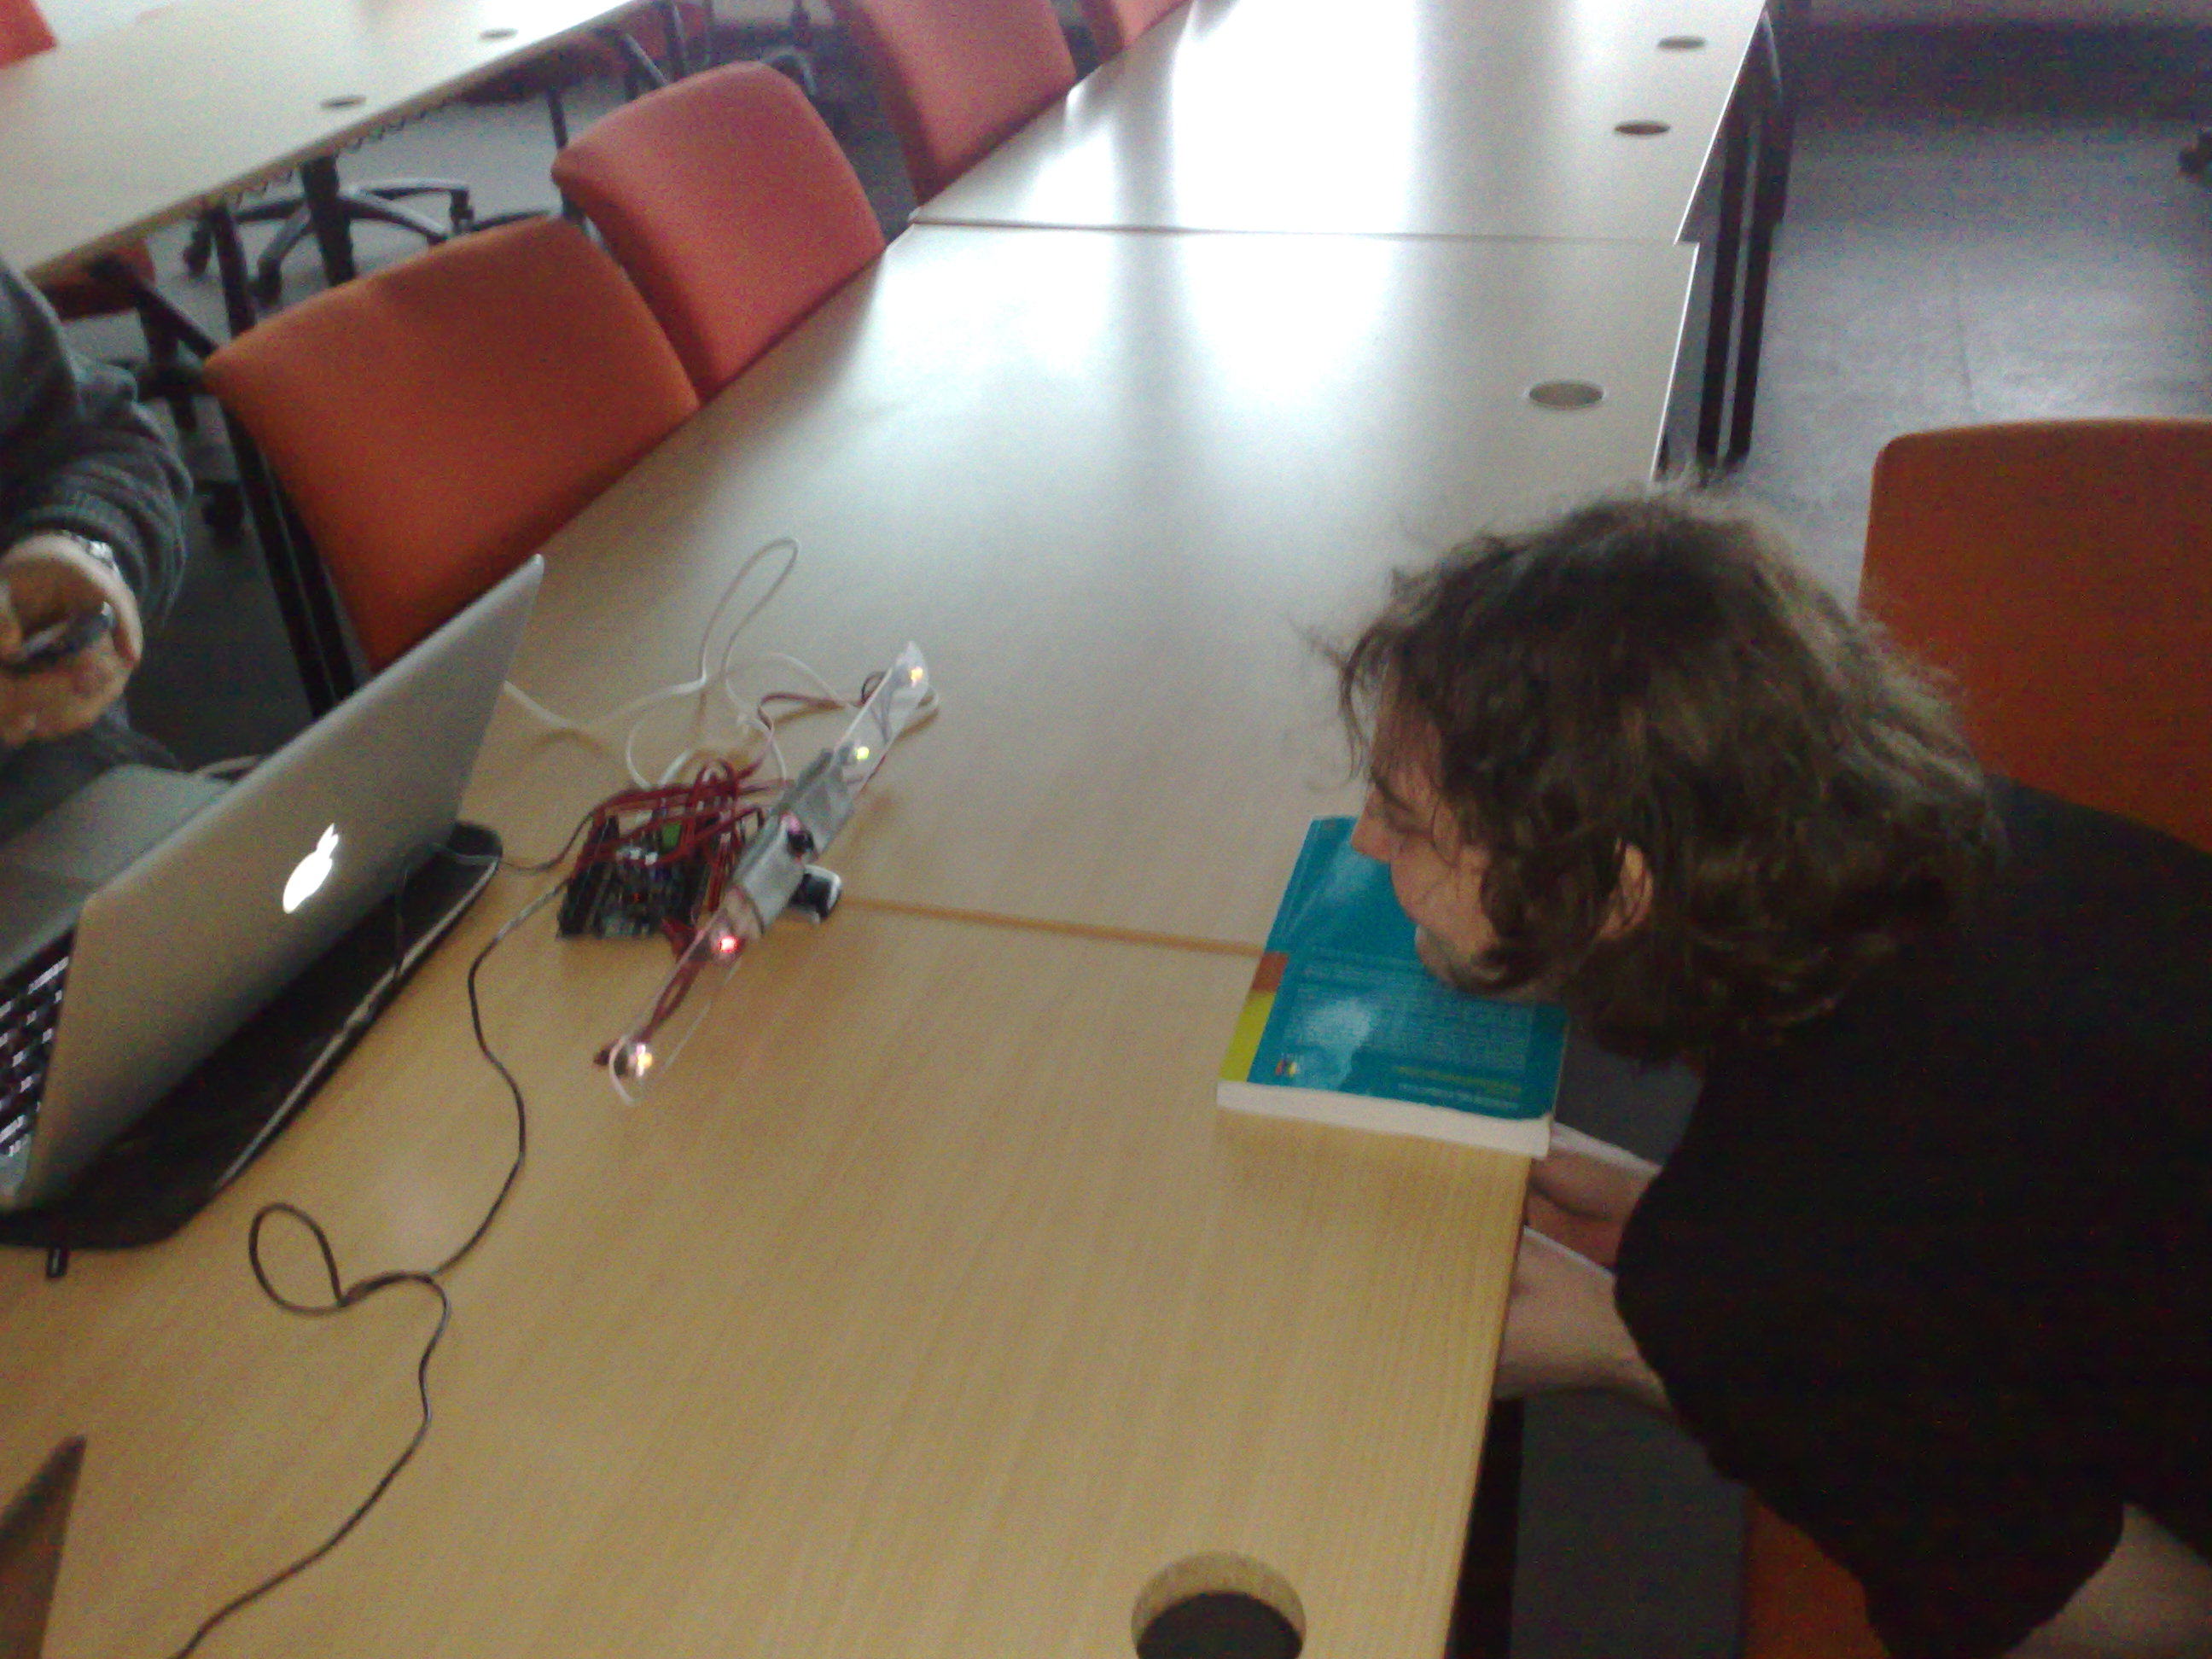
\includegraphics[width=0.8\textwidth]{mikkertest}
\caption{Data gathering on test-subject.}
\label{fig:mikkertest}
\end{figure}


Images were then extracted from the videos every 10 frames using OpenCV and named in such a way it was easy to identify the scenario and the frame it was from.
See Image-grabber.py for details. %proper reference?
Bad images, such as frames were the eyes were obscured or closed, were then manually filtered out and added to an ignore-file.

The corners of the eye and the centre of the pupil were then marked manually using OpenCV and the three points were saved to meta-data files. See EyeMarker.py for details.
This data can be used for feature based learning, though more information such as glints may be desirable.  %proper reference?

For high-dimensional learning, we also needed to separate the eye images.
To do this, eye images were extracted from the larger images using the previously marked points.
To extract the image, the images were loaded and converted to grayscale.
They were then histogram-equalized to broaden the contrast in the image. %skriv noget om effekt på læring?
The eye was then sliced out of the larger image and rescaled to a desired size, such as $20\times 20$, $40\times 40$ or $60\times 60$, and then saved.
For more information see TransformEyeImages.py. %proper reference?

PCA was then run on the eye images %and the feature set
and the results were plotted. See run\_pca.py and pca.py for more information. %proper reference?

After plotting the results, we identified which principal components made the different lights separable and in which cases.
We then tried generating images with different weights on the principal component that made the different points separable to see what effect it had on the image.